%% Erläuterungen zu den Befehlen erfolgen unter
%% diesem Beispiel.

%% Article Template
\documentclass[]{scrartcl}


%% UTF8 Encoding
\usepackage[utf8]{inputenc}
\usepackage[T1]{fontenc}
%\usepackage[margin=5cm]{geometry}% http://ctan.org/pkg/geometry
\usepackage{lmodern}
\usepackage{subcaption}
\usepackage{setspace}
\usepackage[french]{babel}
\usepackage{csquotes}
\usepackage{pdfpages}
% appendix
\usepackage[titletoc]{appendix}

\setstretch{0.99}

%Tabellen mit fixen Breiten
\usepackage{tabularx}

%% Grafik
\usepackage{graphicx} 
\newcommand{\name}{Insta.edit}

%% Links im PDF
\usepackage{hyperref}
\usepackage{csquotes}
\usepackage{rotating}
\usepackage{lscape}
\usepackage{fancyhdr}
\usepackage{float}
\usepackage[titles]{tocloft}
\pagestyle{fancy}
\rhead{
\includegraphics[scale=0.15]{img/insa-logo}}
\chead{\Large -PLD SIE- }
\lhead{Hexanome 4222}

\title{SAP ERP
\subtitle{}
\author{PLD: SIE
Version 1.0}
\date{\today}}


\begin{document}

\maketitle

\begin{figure}[h]
	\centering
  
\includegraphics[width=0.5\textwidth]{img/insa-logo}
	\label{fig:logo}
\end{figure}


\begin{center}
  \begin{tabular}{ | l | r | }
    \hline
    \textbf{Corentin Laharotte}\\ \hline
    \textbf{Cédric Milinaire }\\ \hline
    \textbf{Felix Castillon}\\ \hline
    \textbf{Ousmane Touat}\\ \hline
	\textbf{Grazia Giulia Ribbeni }\\ \hline
	\textbf{Roxane Debord} \\ \hline 
	    \textbf{David Hamidovic}\\ \hline
  \end{tabular}
\end{center}

\thispagestyle{empty}
\pagebreak
\vspace*{10pt}
\tableofcontents
\listoffigures
\newpage
\section{OBJET DU PROJET}
La société SPIE est fondée en 1900 sous le nom de Société parisienne pour l'industrie des chemins de fer et des tramways électriques. Elle devient la Société parisienne pour l'industrie électrique  (SPIE) en 1946. La société SPIE s'occupe de l'étude, la réalisation et la maintenance d'équipements dans différents secteurs : énergie, transport, réseaux extérieurs ,installations électriques, mécanique. La filiale Sud-Est , en particulier, a généré un chiffre d'affaire de 356 Millions d'euros en 2010.\\

La société SPIE souhaite améliorer son activité de maintenance en vue d'une intégration a base de l'ERP SAP. Le but principal est l'amélioration du processus de maintenance. Les types de maintenance auxquels SPIE fait référence son variés: cela va de la maintenance informatique des techniciens sur site jusqu'à la maintenance des infrastructures. \\

En outre, lors de la gestion de la maintenance il faudra prendre en comte, comment:
\begin{itemize}
\item Réaliser les prestations en accord avec le contrat établie, les lignes de conduite de l'entreprise et toutes les lois applicables (fiscalité, environnement, etc.). 
\item Établir un travail de qualité tout en maintenant une quantité garantissant une performance économique\\
\end{itemize}

L'entreprise SPIE Sud Est ayant des secteurs d'activités variés, présente un nombre de données de type différent important. En effet avec au moins 600 interventions par jour, le nombre de données a traiters est important.  De plus ces données proviennent de différents secteurs: commercial, technique ou encore de gestion par exemple. Le but prédominant de ce projet sera d'améliorer la gestion de l'objet métier \textquote{Contrat}. Celui-ci facilite la gestion de la partie forfaitaire  « préventif et curatif » standard et la partie  bon de commande. Cette dernière comprend des événements curatifs exceptionnels et des petits travaux induits.   \\

Finalement. lors de cette étude il faudra particulièrement prendre en comte des technologies déjà mise en place.  Tout d'abord il faudra s'appuyer sur le logiciel Peplesoft, qui permet de faciliter le suivi des activités. Ce logiciel représentant   l'élément central de l'organisationnel informatique de la société il est de la plus haute importance de trouver une solution le prenant en comte.  De plus un facteur important a considérer est la répartition de données. En effet les différents capteurs installé chez les clients collectent des données qui sont centralisé au sein d'un serveur chez un partenaire. \\ 

Pour améliorer l'activité de maintenance en vue d'une intégration a base de l'ERP SAP cette étude traitera les points suivants: 
\begin{itemize}
\item Développement de tableaux de bord de pilotage de réactivité de gestion des contrats de
la maintenance en identifiant au préalable des indicateurs de performance: technique, opérationels et économique.
\item Exploitation de retours d’expérience tant au niveau des clients que de celui des techniciens
\item Psrise en compte des enjeux de sécurité dans le cadre de la réalisation de la maintenance.
En effet, de nombreux équipements, matériels, infrastructures et installations (centrales
nucléaires, systèmes d’alerte incendie de tunnels, centres de contrôle, …) sur lesquels
des actions malveillantes peuvent coûter des vies humaines, nécessitent une sécurité sans
faille. Il s’agit autant de se prémunir contre du sabotage interne que contre des menaces
extérieures. 
\end{itemize}

\newpage
\section{RESULTATS LIVRABLE ATTENDUS: PBS}

Etude préalable : 
\begin{itemize}
\item expression des besoins
\begin{itemize}
\item Dossier de synthèse
\item Benchmarking
\end{itemize}
\item cible fonctionnelle
\begin{itemize}
\item Matrice d'impacts
\item Architecture Applicative Cible v0
\item Matrice des interfaces v0
\end{itemize}
\item Atelier Avanade
\begin{itemize}
\item Matrice FIT/GAP v0
\end{itemize}
\item Construction de la solution
\begin{itemize}
\item Matrice FIT/GAP v1
\item Matrice des interfaces v1
\item Architecture Applicative Cible v1
\end{itemize}
\item Modélisation Détaillée des processus
\begin{itemize}
\item Rapport ARIS
\item Dossier de description de la solution
\end{itemize}
\item Contrôle Qualité
\begin{itemize}
\item Plan d'Assurance Qualité
\end{itemize}
\item [Plan projet]
\end{itemize}
\ \\
Gestion de Projet : 
\begin{itemize}
\item Dossier d'Initialisation
\item Tableau de bord d'avancement
\item Dossier Bilan
\item Ordre du jour
\end{itemize}

\section{OUTILS UTILISES}
Afin de bien organiser notre projet, le choix de bons outils a été important. \\
Nous avons décidé d'utiliser Github pour héberger nos documents. Github est un logiciel de gestion de version Git. Il permet à plusieurs utilisateurs de travailler sur le même document, et gère les conflits lorsque des modifications ont été faites sur les mêmes sections du document. \\
Pour la rédaction de nos rapports, nous avons décidé d'utiliser LateX plutôt que google docs puisque l'ensemble de l'équipe avait plus d'affinités avec ce langage. De plus ce langage peut être facilement combiné à Github. \\
Le suivi de l'avancement de chacun a été réalisé par le logiciel en ligne Trello. Ce logiciel permet de créer des tâches et de les attribuer à chacun. Chaque tâche est assignée à au moins une personne et a une date limite, ce qui permet à chacun de savoir où en est le projet et de s'organiser pour respecter les délais. \\

Pour ce qui est de la gestion de projet, nous avons décidé d'utiliser Microsoft Project qui est un logiciel très complet et qui permet de réaliser tous les documents liés à la gestion de projet. Ce logiciel prend notamment en compte la gestion de la durée de tâches, est capable d'indiquer lorsqu'une ressource est sur-utilisée, et de décaler les tâches ayant subies un retard. 

\section{IDENTIFICATION DES ACTIVITES ET TACHES: WBS}
\subsection{Lises des Activites et des Taches}
\begin{center}
\begin{figure}[H]
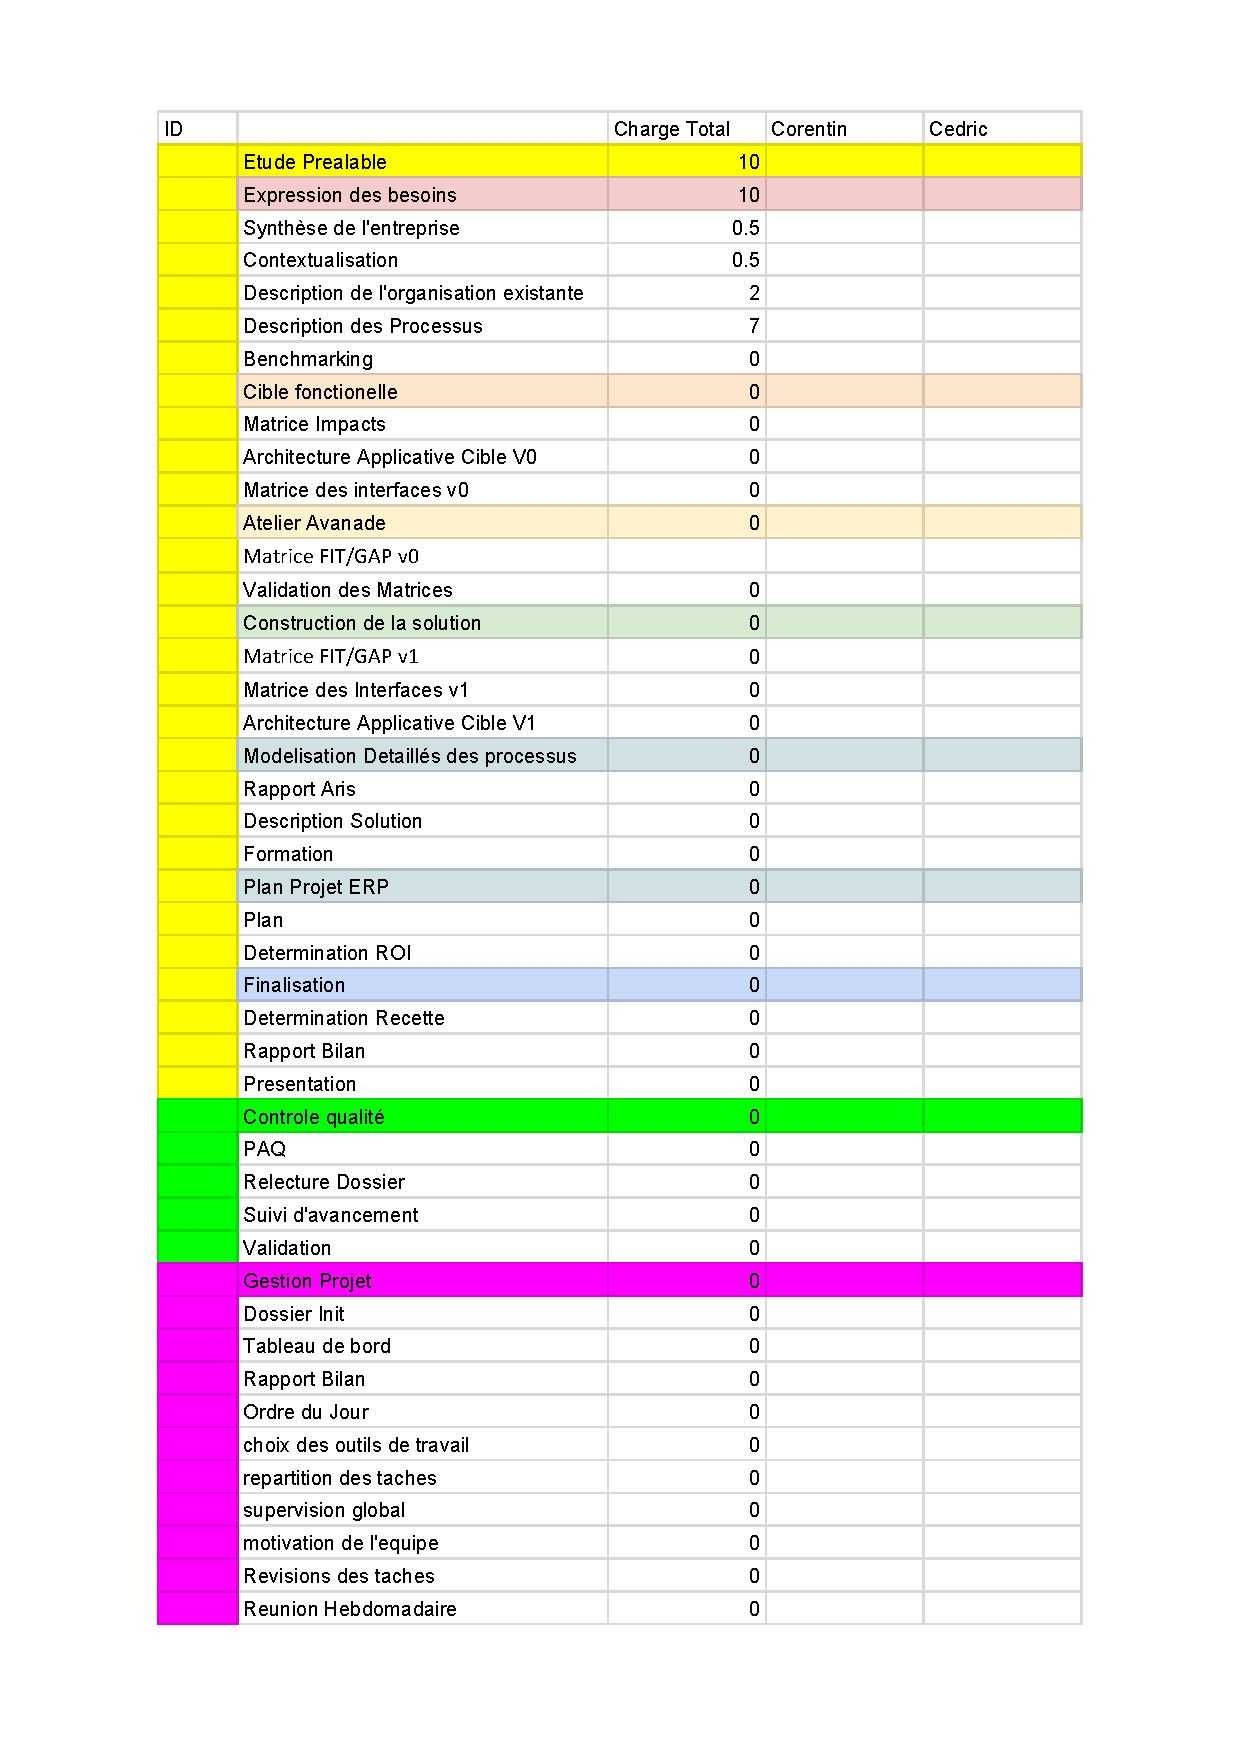
\includegraphics[width=1.15\textwidth]{img/Taches_v0}
\caption{Liste des taches}
\end{figure}
\end{center}
\subsection{Plan de charges}
\begin{center}
\begin{figure}[H]
\caption{Plan de charges}
\end{figure}
\end{center}
\subsection{Diagramme de Gant}
\begin{figure}[H]
\caption{Diagramme de Gantt}
\end{figure}
\section{ORGANISATION DE L'ÉQUIPE:OBS}
\begin{center}
	\begin{tabular}{| l | c | c |}
	\hline
	Role                     & Description & Personne affectée  \\ 	\hline
	Chef de Projet           &             & Cédric Milinaire                   	\\ \hline
	Assistant chef de Projet &             & Corentin Laharotte                  	\\ \hline
	Responsable Qualité      &             & Ousmane Touat                 	\\ \hline
	Responsable Aris         &             & Roxane Debord                 	\\ \hline
	Expert Métier            &             & Grazia Giula Ribbeni                 	\\ \hline
	Expert SAP               &             & David Hamidovic                 	\\ \hline
	Architecte               &             & Félix Castillon  \\ 		\hline
	\end{tabular}
\end{center}

\section{ANALYSE DES RISQUES}
\subsection{Perte de Bobby au court du projet}
Bobby étant le programmeur le plus expérimenté du projet, nous comptons sur lui pour une grande partie des taches. S’il lui arrive un contretemps et qu’il vient à nous quitter, nous devrions trouver des alternatives à cela. Nous ne pouvons faire appelle à d’autre programmeur pour palier à son manque. Les compétences en développement du chef de projet lui permettront de prendre une partie du travail laissé par Bobby. Il en résultera un retard certain mais moins important que prévu. Le retard serait de 10 à 40 jours en fonction de la date de départ.


\begin{appendices}
\end{appendices}
\end{document}
